\chapter[Metodologia]{Metodologia}

\section{Metodologia}

O desenvolvimento da aplicação foi feito de maneira individual, e para organização do desenvolvimento foi feito primeiro um levantamento de requisitos. Os requisitos da aplicação foram esses:

\begin{enumerate}

    \item É necessário armazenar um número limitado de questões e eventos das maratonas UnB com     atualização não frequente
    \item O visitante do site deve ter capacidade de enviar sua solução em código para que ela seja julgada, e em pouco tempo ele deve receber o veredicto de sua submissão, caso passe em todos os testes o sistema deve deixar claro que seu código foi aceito, caso contrário o sistema deve     apresentar uma mensagem exemplificando o erro como TLE, MLE, RE.
    \item O visitante do site deve conseguir ter acesso aos problemas e eventos por um site, a tutoriais e dicas das questões, sendo que as dicas sejam frases que auxiliam o visitante na resolução do problema e o tutorial um guia completo sobre uma abordagem de solução do problema
\end{enumerate}

Dentro desses requisitos básicos as tarefas foram separadas em épicos e quebradas em tarefas menores, dentre todas as tarefas menores o nível de priorização foi feita com base em meu conhecimento em tecnologias, os requisitos que eu tinha conhecimento que poderiam ser cumpridos tiveram uma prioridade menor, pois caso algum requisito fosse mais difícil ou exigisse mais tempo de estudo para ser cumprido eu poderia avaliar alternativas.

Os requisitos citados acima estão feitos de uma maneira mais ampla e precisam ser quebrados em tarefas, para um melhor detalhamento e facilidade na execução.

\subsection{Épico de armazenamento de questões}

É necessário armazenar um número limitado de questões das maratonas UnB com atualização não frequente

\subsubsection{Tarefas}

\begin{enumerate}
    \item Criação de um banco de dados para armazenar questões e eventos.
          \begin{enumerate}
              \item As questões devem possuir título, enunciado, tempo limite de execução, limite de memória utilizado pelo programa, lista de tags que categorizam o problema, ID predefinido para localização das questões e identificação , lista de inputs e outputs de teste de teste.
              \item Os eventos devem possuir uma data que identifica quando o evento aconteceu, um nome e uma lista de problemas, tal como o rótulo do problema naquele evento ex: "Questão A"
          \end{enumerate}
    \item Estabelecer uma relação entre as questões e os problemas, que deixe claro de qual evento aquele problema foi originado e a lista de problemas de um evento.
    \item Disponibilizar um recurso para o armazenamento de novos eventos e novos problemas
    \item Disponibilizar um recurso para recuperação de problemas e eventos
    \item Disponibilizar um recurso para busca de eventos e problemas
\end{enumerate}



\subsubsection{Execução}

Para esse épico e essas tarefas optei por utilizar um banco de dados NoSQL o MongoDB seguindo sua documentação, também utilizei um sistema em NodeJS que faz a gestão do banco e exposição de uma API REST, utilizando a linguagem de programação Typescript.O motivo da escolha desse banco de dados foi pela flexibilidade e compatibilidade com o sistema Node, o intuito do trabalho em geral é ser simples e convidativo para novos usuários que pretendem contribuir, portanto a mesma tecnologia e linguagem utilizada para o front da aplicação foi utilizada no backend da aplicação.A principal razão para utilização de Typescript como linguagem de programação é pelo fato da linguagem ser fortemente tipada, portanto boa parte dos erros podem ser capturados pelo próprio compilador. Apesar de ser uma abordagem mais incisiva em relação ao desenvolvimento, que obriga o usuário a declarar o tipo das suas funções e objetos, ela traz facilidades para análise estática e resolução de bugs, e visto que o foco da aplicação é ser convidativa para novos contribuidores a utilização de typescript pode alertar erros comuns de iniciantes.

\subsection{Épico do juiz online}

O visitante do site deve ter capacidade de enviar sua solução em código para que ela seja julgada, e em pouco tempo ele deve receber o veredicto de sua submissão, caso passe em todos os testes o sistema deve deixar claro que seu código foi aceito, caso contrário o sistema deve apresentar uma mensagem exemplificando o erro como TLE, MLE, RE.

\subsubsection{Tarefas}
\begin{enumerate}
    \item Criação de um sistema que recebe um código em formato de arquivo, com o armazenamento persistente desse arquivo feito de maneira opcional
    \item Armazenamento de entradas e saídas esperadas de problemas, com um código pré-definido que poderá ser utilizado por outros serviços da aplicação.
    \item Criação de sistema que executa esse arquivo em uma linguagem de programação, dentre elas as principais linguagem que devem ser suportadas são, Java, C, C++ e Python, a execução deve possuir um tempo deve ter um tempo limite, e comparar as saídas esperadas do programa executado com as saídas esperadas do servidor, após a execução o sistema deve retornar um veredito para o usuário, como descrito no épico acima
\end{enumerate}

\subsubsection{Execução}

A execução desse épico ainda não foi feita e está planejada para ser realizada utilizando ferramentas similares às dos outros módulos da aplicação. Um servidor será feito utilizando NodeJS com Typescript de linguagem e para julgar as questões será utilizado alguma forma ainda não definida de isolar um ambiente que executa os códigos, será feito um monitoramento dos recursos utilizados, como memória, e o tempo gasto para a execução do problema. Esse módulo da aplicação será responsável também por armazenar as entradas e saídas dos problemas para entregar o veredito do código executado

\subsection{Épico de interface de usuário}

O visitante do site deve conseguir ter acesso aos problemas e eventos por um site, a tutoriais e dicas das questões, sendo que as dicas sejam frases que auxiliam o visitante na resolução do problema e o tutorial um guia completo sobre uma abordagem de solução do problema

\subsubsection{Tarefas}
\begin{enumerate}

    \item Criação de um frontend que se comunica com os outros serviços e disponibilize ao usuário as informações citadas no épico acima
          \begin{enumerate}
              \item Criação de uma tela com as informações do problema, como enunciado, título, tempo limite, limite de memória, nessa tela deverá ser possível o usuário selecionar um arquivo de seu computador e enviar ao sistema para ser julgado, esta tela deverá suportar o formato LaTEX vindo como string do servidor e deverá suportar a inserção de tags HTML como tags de imagem e de estilização de texto.
              \item Criação de uma tela com o tutorial da questão, essa tela deverá suportar o formato LaTEX vindo como string do servidor e deverá suportar a inserção de tags HTMLcomo tags de imagem e de estilização de texto.
              \item Criação de uma tela com detalhes do evento, contendo o título do evento, data e a lista de problemas que ocorreu naquele evento, com um link com a página da respectiva questão
              \item Criação de uma tela com a lista de problemas, onde deve ser possível buscar problemas pelo título, título do evento em que ele aconteceu ou tags do problema.
              \item Criação de uma tela com a lista de eventos, onde deve ser possível buscar eventos pelo seu título e ordenar os resultados pela data do evento ou ordem alfabética.
          \end{enumerate}
    \item Criação de funções que estabeleçam comunicação com os outros serviços da aplicação
          \begin{enumerate}
              \item Criação de uma funções que faça uma busca dos problemas no serviço que faz o armazenamento dos problemas ou que recupere um único evento com todos os seus detalhes
              \item Criação de uma função que faça uma busca dos eventos no serviço que faz o armazenamento dos eventos ou que recupere um único evento
              \item Criação de uma função que envie o arquivo de execução do usuário para o serviço que julga as questões, mostrando para o usuário o resultado de sua submissão
          \end{enumerate}
\end{enumerate}

\subsubsection{Execução}

Para realização desse épico foi utilizado uma aplicação em React com NodeJS, utilizando Typescript como linguagem, o motivo para a escolha dessas tecnologias foi a familiarização com as mesmas e a flexibilidade e facilidade de criação e reutilização de componentes

\section{Ferramentas utilizadas}

\subsection{Ferramenta de versionamento}

O desenvolvimento dos resultados parciais foi feito utilizando a ferramenta de versionamento git, e o github, um hub da ferramenta que possibilita o versionamento da aplicação.

\subsection{Hardware}

Foram utilizadas 2 máquinas diferentes para o desenvolvimento e o compartilhamento do código foi feito com o auxílio da ferramenta de versionamento. Uma máquina possui o sistema Ubuntu 20.04.3 LTS e a outra um macOS Big Sur 11.5.2.

\subsection{Principais softwares}

Os principais frameworks e softwares utilizados para o desenvolvimento foram o Node.js v12.10.0,  React v17.0.2 e Bootstrap v2.0.0-beta.4. Foram utilizados outros softwares como dependências dentro do node que estão listados nos arquivos \textit{package.json} dos respectivos projetos.

\subsection{Fluxo de trabalho}

O trabalho do desenvolvimento foi bastante flexível por se tratar de um desenvolvimento individual, com apenas um desenvolvedor a flexibilidade de escolha do que desenvolver foi maior.

Uma das principais preocupações durante o desenvolvimento foi a manutenibilidade do software, futuramente o software poderia ser continuado por outras pessoas, que dominam ou não as tecnologias escolhidas, portanto a documentação da API, documentação de dependências e como rodar o software foram feitas pensando nisso. Assumindo que os futuros mantenedores tenham um conhecimento básico em REST API, da api desenvolvida para comunicação com o banco de dados da aplicação, API que é utilizada na interface da aplicação para exibição dos problemas e eventos.

A escolha de ordem de desenvolvimento não foi aleatória, foram priorizados os pontos que eu menos dominava e menos tinha conhecimento, para avaliar a viabilidade e estimar o tempo de desenvolvimento de certas funcionalidades mais precisamente. Primeiramente foi feito a API e a conexão com o banco de dados MongoDB. Um ponto avaliado foi a compatibilidade das bibliotecas com o typescript, que foi a linguagem escolhida para desenvolver com Node.js, por não ser a linguagem mais comum, algumas bibliotecas podem apresentar problemas de funcionamento ou necessitar de adaptações para sua utilização. Um exemplo disso é a biblioteca \textit{mongose}, essa biblioteca é bem famosa para projetos utilizando Node.js, com javascript de linguagem, e mongodb, ela facilita ao abstrair algumas etapas na conexão com o banco de dados, porém ao utilizar a biblioteca alguns problemas foram encontrados durante o desenvolvimento, a conexão com o banco não foi estabelecida e alguns tipos de dados nas interfaces das funções estavam obsoletos, impedindo o funcionamento da aplicação. Por conta disso o desenvolvimento foi feito utilizando o driver do próprio mongodb. Esse tipo de escolha foi feita em todo projeto, a utilização de bibliotecas externas foi evitada ao máximo, evitando excessivas abstrações, e quando utilizadas a compatibilidade com typescript foi um critério crucial para utilização.

O segundo passo foi a interface, na interface um ponto importante foi a utilização da biblioteca bootstrap, a motivação da escolha dessa biblioteca e utilização de seus componentes foi o fato dos componentes possuírem um design agradável, sua compatibilidade com typescript, outro ponto importante para a escolha é que ela possui vários componentes muito utilizados no desenvolvimento web, por se tratar de uma aplicação simples esses componentes ajudariam bastante. Para auxiliar o desenvolvimento foi utilizado a documentação oficial da biblioteca React Bootstrap com exemplos de utilização dos componentes. Um dos requisitos levantados foi a compatibilidade da interface com LaTEX, para escrita de funções e expressões matemáticas nos problemas armazenados no servidor. Para isso outra biblioteca importante utilizada foi o React LaTEX Next, com ela os textos com componentes LaTEX são renderizados, podendo conter até tags HTML de estilo.

\section{Arquitetura}

A arquitetura geral escolhida para execução do projeto foi a de micro-serviços, separando a aplicação em módulos com pequenos conjuntos de responsabilidades individuais. A arquitetura de micro-serviços consiste em variados softwares que trabalham de forma independente. Em contraposição, existe a abordagem monolítica na qual o serviço concentra todas as responsabilidades do software. De fato, a abordagem monolítica é bastante eficaz para um sistema pequeno, pois facilita o deploy e desenvolvimento da aplicação; no entanto, na medida em que cresce a concentração de funcionalidades em um só sistema, agrava a complexidade do código, dificultando seu entendimento e manutenção, conforme afirma Namiot (\citeyear{namiot_d:OMSA}) em On Micro-services Architecture.

A separação nesses módulos visa a flexibilidade de escalar os micro serviços de forma independente: ``[\dots] Com a arquitetura monolítica, não é possível escalar cada componente de maneira independente'' \cite[tradução nossa]{namiot_d:OMSA}[p.24]\footnote{``[\dots] With a monolithic architecture, we can not scale each component independently''}. Outro benefício na separação das responsabilidades em 2 sistemas independentes é o desenvolvimento de novas features, manutenção e possível troca de framework ou de tecnologia presente no software para algo mais adequado ou algo mais novo. Em uma arquitetura monolítica, mudar o código pode se tornar muito difícil dependendo do tamanho e complexidade da aplicação, coadunamente, Namiot afirma: ``[\dots] Com a arquitetura monolítica, é muito difícil (se lê impossível) realizar mudanças.''\cite[tradução nossa]{namiot_d:OMSA}[p.24]\footnote{``[\dots] With the monolithic architecture, it is very difficult (read impossible) to change it.''}

A arquitetura se resume a dois micro serviços com responsabilidades específicas:
\begin{enumerate}
    \item Prover informações das questões.
    \item Executar e julgar códigos.
\end{enumerate}

A primeira responsabilidade é fazer uma ponte de comunicação com o banco de dados. Nesse módulo, é feito o cadastro de questões e eventos dentro do banco, a recuperação desses dados e outras necessidades agregadas, como busca por questões ou busca por eventos.

O segundo serviço é responsável por receber arquivos com códigos, executá-los e retornar um veredito. Ao receber um arquivo ou um texto contendo o código, ele se responsabiliza em executa-lo em uma linguagem de programação escolhida previamente, passar o programa executado por diversas entradas diferentes e comparar os resultados obtidos com os resultados esperados, retornando o veredito. E.g. WA, veredito retornado quando as saídas do código enviado se diferem das esperadas.

As duas competencias citadas funcionam bem de maneira independente, caso o banco de questões seja alterado, trocando a maneira em que é armazenado o enunciado das questões, isso não afeta o micro serviço que julga os códigos dos usuários; adicionalmente, caso sejam adotados novos métodos para julgar as questões, o módulo que armazena as questões também não será afetado.

Os serviços descritos são simples e conseguem abranger todos os requisitos da aplicação. Diante do exposto, o padrão de abordagem escolhido para comunicação entre os micro serviços e a aplicação foi a de acesso direto, onde os micro serviços se comunicam diretamente com a aplicação - é dizer, a interface de usuário. Esse padrão também é discutido por Namiot (\citeyear{namiot_d:OMSA}). A Figura \ref{fig:architecture} abaixo representa a arquitetura descrita e seus respectivos módulos:

\begin{figure}[h]
    \centering
    \caption{Arquitetura dos micro serviços da aplicação}
    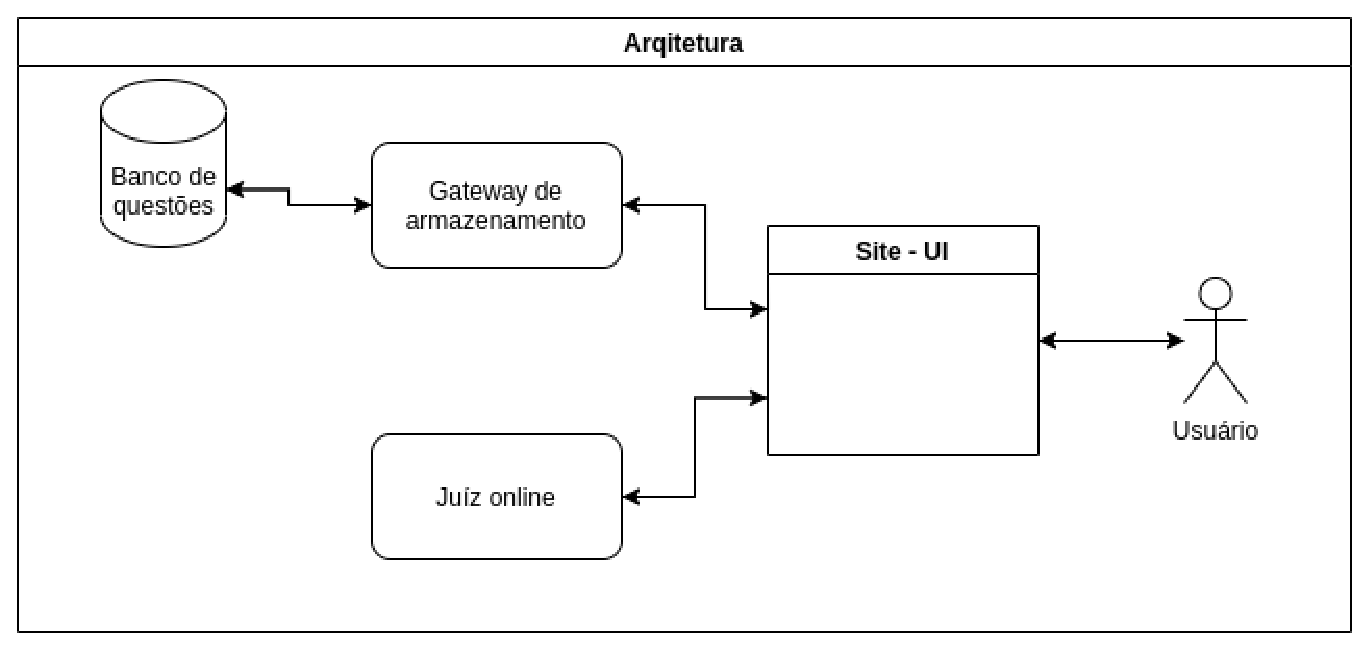
\includegraphics[keepaspectratio=true,scale=0.6]{figuras/arquiteture.eps}
    \label{fig:architecture}
\end{figure}
\begin{center}
    Fonte: elaboração nossa
\end{center}

Conforme pode ser observado, o primeiro módulo é representado como ``Gateway de armazenamento'' na figura. Ele faz a comunicação bidirecional com um banco de dados e com a aplicação, representada como ``Site - UI''. O segundo módulo descrito é representado como ``Juiz online'', ele faz uma comunicação bidirecional com a aplicação. Dentro dos requisitos da aplicação não se torna necessário o armazenamento das informações de submissões e vereditos, a partir desse fato, não necessariamente esse módulo utiliza um banco de dados, no entanto, pode ocorrer utilização de um caso os requisitos da aplicação mudem.